\section{Scenarios as Message Sequence Charts}

Unlike labeled transition systems, that intrinsically model the behavior of a single agent (even if a composed one), scenarios explicitly illustrate interactions among multiple agents. The scenarios we use in this thesis are a syntactic subset of Message Sequence Charts (MSC)~\cite{ITU:1996} (see Fig.~\ref{image:train-scenario-all-agents} for example). To keep the models usable by end-users, however, we use only a small subset of their features. In its simplest form, a MSC is composed of vertical lines representing timelines associated with agents and horizontal arrows representing interactions among agents, also called \emph{events}. Following the modeling of agents of the previous section, events are synchronously sent and received by interacting agents (we also use the terms \emph{controlled} and \emph{monitored} events, respectively). As already stated in previous section, we assume that an event label uniquely determines the latter agents. 

We consider \emph{positive} scenarios, as examples of behaviors that the system should exhibit, in the next section and \emph{negative} scenarios, behaviors that the system must avoid, in the following one. Subsequent sections will then discuss ways of managing multiple positive and negative scenarios. 

\subsection{Positive scenarios\label{subsection:background-positive-scenarios}}

The semantics of MSCs in this thesis is defined in terms of labeled transition systems, following~\cite{Uchitel:2003}. More precisely, MSCs are given a trace semantics, which is captured with LTSs, as in previous section. However, given a MSC, two kinds of traces can be considered: those from the local perspective of a single agent, and those from the global perspective of the composed system. We discuss each of these views in turn.

As time in a MSC is represented top-down, the order in which events are sent and received along a particular timeline defines a total order. Therefore, from the perspective of a single agent, a MSC defines only one trace; precisely, one \emph{maximal} trace (that is, with all events to which the agent participates) and all its prefixes. For example, the traces seen by the \artifact{Controller} agent in the MSC of Fig.~\ref{image:train-scenario-all-agents} are precisely captured by the LTS of Fig.~\ref{image:local-traces-lts}. Given a MSC $M$ and an agent $Ag$, we denote such an LTS by $M_{\downarrow Ag}$.

\vspace{0.5cm}
\begin{figure}[H]\centering
\scalebox{0.45}{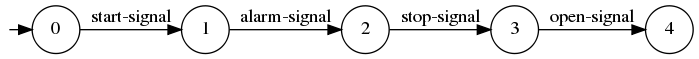
\includegraphics{src/2-framework/images/local-trace}}
\caption{LTS capturing the traces of the MSC of Fig.~\ref{image:train-scenario-all-agents} from the local point of view of the \artifact{Controller}.\label{image:local-traces-lts}}
\end{figure}

When considering the composed system, two interpretations co-exist. In the former, a reasoning similar to the one for agents is applied. Indeed, one can consider that a MSC defines a \emph{maximal} trace in the composed system, with all events in a top-down ordering. In the example at hand, such a trace would be \artifact{<start-signal, start, alarm-pressed, \ldots, open>}. Making so amounts to consider that a MSC defines a total order among all events; this leads to a simple and straightforward, yet limited, trace semantics of MSCs.

However, when considering concurrent systems, considering a partial ordering among events often appears more adequate~\cite{ITU:1996, Uchitel:2003}. Consider for example the events \artifact{start-signal} and \artifact{alarm-pressed} at beginning of the MSC. These two events model unrelated phenomena between different agents, and can therefore hardly be considered timely ordered (e.g. maybe does the passenger push the alarm button when the \artifact{start-signal} is already sent but before \artifact{start} has been propagated? or even before \artifact{start-signal}?, and so on.). Assuming a partial ordering of events leads to a more general trace semantics of MSCs (more general in the sense that it includes traces defined under a total ordering assumption), but also more complex. In this case, the traces defined by a MSC are the \emph{linearizations} of the partial order among events. We do not formalize the structure of Message Sequence Charts and their linearizations here, and refer the reader to~\cite{Uchitel:2003} for such a mathematical characterization. However, we state the relations that hold between the set of traces of the system -- under a total or a partial order assumption -- and those obtained by composing agent traces:

\begin{equation}
\label{equation:msc-composition}
\mathcal{L}_{total}(M) \subseteq \mathcal{L}_{partial}(M) = \mathcal{L}(M_{\downarrow Ag_1} \parallel \ldots \parallel M_{\downarrow Ag_n}) = \mathcal{L}_{arch}(M)
\end{equation}

The left part simply states that traces under a partial order assumption certainly include those under a total order one, which is expected. The right part provides a simple way of computing all linearizations of a MSC as an (acyclic) transition system, through LTS composition (the reason we call it $\mathcal{L}_{arch}$ will become clear in a next section). Such a LTS is illustrated in Fig.~\ref{image:msc-linearizations} for the MSC of Fig.\ref{image:train-scenario-all-agents} that accepts six different linearizations, due to the possible interleaving of its first four events. By construction, such a LTS has only one initial state (the leftmost one) and only one terminating state (the rightmost one). This allows us to loosely refer to \emph{the} terminating state of an MSC (at least, of the LTS capturing its traces) with a precise underlying meaning.

\aside{The reader familiar with the related literature may wonder here if some of these traces should not be considered as \emph{implied} scenarios. Strictly speaking, that is, according to the definition of an implied scenario given in~\cite{Uchitel:2004}, they are not. One could also think that the initial scenario is problematic, for example because the passenger monitors the fact that the train moves, a fact that could be modeled explicitely with additional events. While this latter remark actually makes sense, we argue that always dealing with scenarios that do not present possible interleaving amounts to hide -- or even deny -- the intrinsic concurrent nature of multi-agent system, the one which by its complexity triggers the need of modeling such systems. We further discuss these questions in section \ref{section:background-discussion}.}

\begin{figure}\centering
\scalebox{0.31}{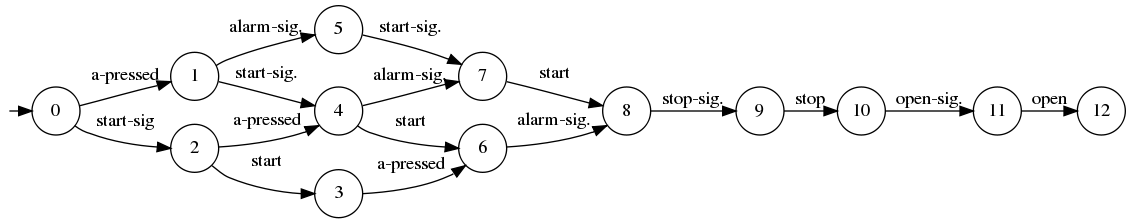
\includegraphics{src/2-framework/images/linearizations}}
\caption{LTS capturing all event linearizations of the MSC of Fig.~\ref{image:train-scenario-all-agents}. Here, \artifact{alarm-pressed} is abbreviated as \artifact{a-pressed} and \artifact{sig.} stands for \artifact{signal}. \label{image:msc-linearizations}}
\end{figure}

\subsubsection*{Multi-view model consistency}

The semantics of a single MSC in terms of agent and system traces can now be explicitly related to the notions of agent and system behavior from Section~\ref{section:background-agents-system-behaviors}. This amounts to define consistency rules between them, and explains the similitude between definitions \ref{equation:system-composition} and \ref{equation:msc-composition}.

Consider a system $S$ composed of $n$ agents whose behavior is modeled by the LTSs $Ag_1$ to $Ag_n$. Let $M$ denote a MSC illustrating interactions between them. We say that $M$ is \emph{consistent} with $S$ -- or, more accurately, that $M$ and $S$ \emph{are} consistent -- if the following conditions hold:

\begin{itemize}
\item $M$ and $S$ are \emph{architecturally} consistent,
\item $\mathcal{L}(M_{\downarrow Ag_i}) \subseteq \mathcal{L}(Ag_i)$ for each agent $Ag_i$, and
\item $\mathcal{L}(M_{\downarrow Ag_1} \parallel \ldots \parallel M_{\downarrow Ag_n}) \subseteq \mathcal{L}(Ag_1 \parallel \ldots \parallel Ag_n)$
\end{itemize}

The first condition is not formalized but simply requires the MSC and the system to agree on the set of agents (a MSC may actually illustrate interactions among a proper subset of system agents) and their respective interfaces (labels along a timeline are a subset of the alphabet of the corresponding agent). The second condition states that the traces defined by a timeline in the MSC must be traces accepted in the LTS modeling the behavior of the corresponding agent. The third condition states that all linearizations of the MSC must be accepted traces of the LTS modeling the behavior of the composed system. Note that, under architectural consistency, the second condition implies the third one~\cite{Uchitel:2003}. Also, these inter-model consistency rules are given for the general model with partial ordering and therefore guarantee consistency under total ordering as well. Last, but not least, stated conditions restrict consistent MSCs to those starting in the system initial state.

\subsection{Negative scenarios}

While positive MSCs model examples of behavior that the system is expected to exhibit, it is often convenient to be able to model the counterpart, that is examples of behavior that the system is expected (even required) \emph{not} to exhibit. Such proscribed behaviors are illustrated with negative MSCs~\cite{Uchitel:2004}. A negative MSC is simply a scenario whose last event is proscribed, as depicted by a crossed arrow below a dashed line. An example is given in Fig.~\ref{image:train-negative-scenario}, where the \artifact{Controller} may not open doors immediately after having started the train.

\begin{figure}[H]\centering
\scalebox{0.75}{
  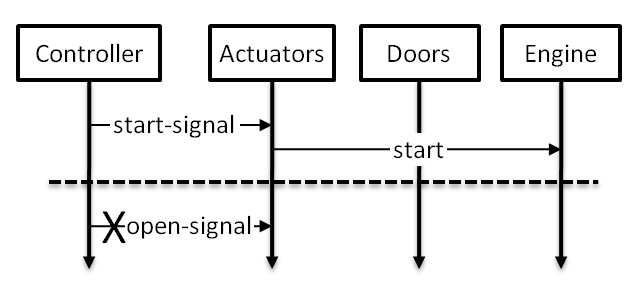
\includegraphics[trim=2mm 2mm 2mm 2mm, clip]{src/2-framework/images/train-negative-scenario}
}
\caption{A negative scenario illustrating that the controller may not open doors after having started.\label{image:train-negative-scenario}}
\end{figure}

More precisely, a negative MSC is a pair $(P,e)$ where $P$ is a positive MSC and $e$ is a single event (given our simplifying assumption, the latter event can simply be denoted by its label $l = label(e)$). The positive scenario $P$ is called the $precondition$ and $e$ the \emph{proscribed event}. The intuitive semantics is that, once the precondition has occurred from the system initial state, $e$ may not be the (very) \emph{next} event in the system. We make this semantics fully precise now. A negative MSC $N = (P,e)$ defines a set of traces as follows:

\begin{align*}
\mathcal{L}_{total}(N)   &= \{~w.l \mid w \in \mathcal{L}_{total}(P) \wedge l = label(e)~\} \\
\mathcal{L}_{partial}(N) &= \{~w.l \mid w \in \mathcal{L}_{partial}(P) \wedge l = label(e)~\}
\end{align*}

That is, traces of a negative MSC are traces of the precondition (provided a consistent choice of partial or total ordering) concatenated with the label of the proscribed event. Note that such a definition implies that the precondition must occur completely for the proscribed event to be taken into account. In other words, partial orderings between the proscribed event and those in the precondition are never considered. This is the intended meaning of the dashed line separating them~\cite{Uchitel:2004}. 

\subsubsection*{Multi-view model consistency}

Similarly to positive MSCs, we state conditions for a negative MSC $N = (P,e)$ and a system $S = (Ag_1 \parallel \ldots \parallel Ag_n)$ to be consistent, as follows:

\begin{itemize}
\item $N$ and $S$ are \emph{architecturally} consistent,
\item $P$ and $S$ are consistent, and
\item $\mathcal{L}_{partial}(N) \not\subseteq \mathcal{L}(Ag_1 \parallel \ldots \parallel Ag_n)$
\end{itemize}

The first condition is similar to what has been said previously for positive MSCs. The second enforces the precondition to be a consistent (positive) MSC. The last one states that the system may not exhibit any trace captured by the negative MSC. Here as well, inter-consistency rules are given for the general model with partial ordering and imply consistency in the stronger model.

\subsection{Scenario collections}

Systems are generally illustrated with multiple positive and negative scenarios. The most straightforward way of doing so is through scenario collections $Sc = (S^+,S^-)$ where $S^+$ and $S^-$ are (possibly empty) sets of positive MSCs and negative MSCs, respectively. It is straightforward, yet useful, to extend the notions of language and consistency of scenarios to collections of them. 

The positive and negative languages defined by a scenario collection $Sc = (S^+,S^-)$ are simply defined via the union on languages:

\begin{align*}
\mathcal{L}^+(Sc) = \bigcup_{P \in S^+} \mathcal{L}(P) \\
\mathcal{L}^-(Sc) = \bigcup_{N \in S^-} \mathcal{L}(N)
\end{align*}

Also, a scenario collection and a system are said to be consistent if and only if each positive and each negative MSC of the collection is itself consistent with the system. We extend this to the consistence of the collection of scenarios itself as follows: two sets of positive and negative scenarios, $S^+$ and $S^-$, are consistent with each other if there exists a system which is consistent with them taken as a collection $Sc = (S^+,S^-)$. A necessary condition for a scenario collection to be consistent (but not sufficient, because architectural consistency is not taken into account here) is the disjointness of positive and negative traces:

\begin{center}
$Sc = (S^+,S^-)$ is consistent only if $\mathcal{L}^+(Sc) \cap \mathcal{L}^-(Sc) = \emptyset$
\end{center}

Note that, by definition, a collection cannot be consistent with a system unless all scenarios start in its initial system state. Also, a (finite) scenario collection is hardly complete in practice, in the sense that it cannot describe all system behaviors (most system accept an infinite number of traces, through loops). Last, multiple scenarios starting in the same initial state imply a lot of redundancy in system descriptions, which renders refactoring difficult in practice. High-level Message Sequence Charts (hMSCs), introduced in the next section, provide a mean to tackle these three problems.

\subsection[Flowcharting scenarios in high-level MSCs]{Flowcharting scenarios in high-level Message Sequence Charts\label{section:background-hmsc}}

High Level Message Sequence Charts are directed graphs where each node refers to a MSC (named \emph{basic} MSC here, bMSC for short) or a finer grained hMSC~\cite{ITU:1996}. Outgoing edges of a node capture its possible continuations, allowing the user to introduce sequences, alternatives and loops, to reuse small MSC fragments, and so on. An hMSC also has an initial starting point that indicate the initial system state. An example of hMSC is given in Fig.~\ref{image:train-hmsc}. A trace semantics can be given to high-level MSCs, and captured in terms of LTSs. This amounts to answering the question \emph{what traces are accepted by (or defined by) a hMSC?} We summarize here, and slightly extend, the characterization given in~\cite{Uchitel:2004}.

\begin{figure}\centering
\scalebox{0.66}{
  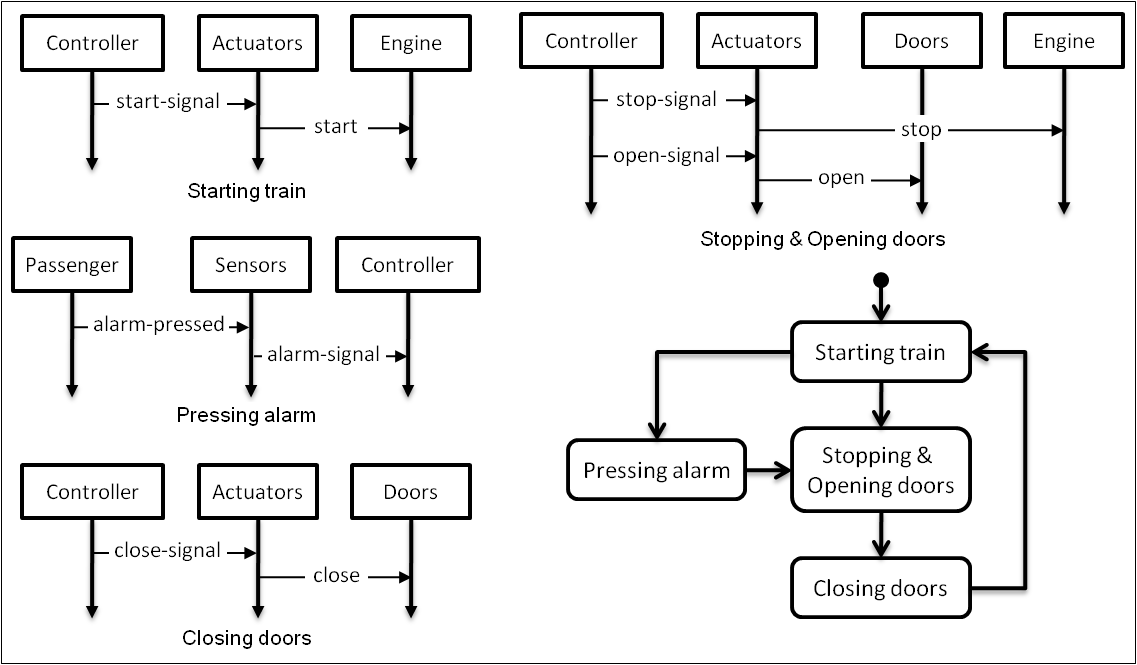
\includegraphics[trim=2mm 2mm 2mm 2mm, clip]{src/2-framework/images/train-hmsc}
}
\caption{A high-level Message Sequence Chart for the train system.\label{image:train-hmsc}}
\end{figure}

In addition to the partial or total ordering of events in bMSCs, two interpretations co-exist about how a system evolves from a bMSC to another inside a hMSC. The first one, called \emph{strong sequential composition}, is to assume that all agents wait until all events of a bMSC have occurred before moving on to the next one. This implies that there is an implicit synchronisation scheme used by agents to know when a scenario has been completed. The other one, \emph{weak sequential composition}, does not make such an assumption and allows an agent to move from a bMSC to another one without having to synchronize with the other agents. Given the independence between assumptions of partial/total event ordering and weak/strong sequential composition, four combinations actually exist. To keep things simple enough, and because they lead to strange concurrency models\footnote{in particular, one can check that such models are sentitive to bMSC concatenation and decomposition}, we don't consider partial (resp. total) ordering with strong (resp. weak) sequential composition. In the sequel, therefore, strong (resp. weak) sequential composition implies total ordering (resp. partial) of MSC events.

The trace analysis for hMSCs is very similar to what has been done for MSCs, and therefore leads to language relations similar to the ones given for the latter in Section~\ref{subsection:background-positive-scenarios} (see equation~\ref{equation:msc-composition}):

\begin{equation}
\mathcal{L}_{strong}(H) \subseteq \mathcal{L}_{weak}(H) \subseteq \mathcal{L}(H_{\downarrow Ag_1} \parallel \ldots \parallel H_{\downarrow Ag_n}) = \mathcal{L}_{arch}(H)
\label{equation:hsmc-traces-by-agent-composition}
\end{equation}

The set of traces $\mathcal{L}_{strong}(H)$ and $\mathcal{L}_{weak}(H)$ are easily explained by considering scenarios ``built'' by the hMSC. Consider a finite path in the hMSC; concatenating the bMSCs along this path ``builds'' a single MSC. For example, concatenating \artifact{Starting train}, \artifact{Pressing alarm} and \artifact{Stopping \& Opening the doors} in the hMSC of Fig.~\ref{image:train-hmsc} leads to the MSC of Fig.~\ref{image:train-scenario-all-agents}. From results in Section~\ref{subsection:background-positive-scenarios}, such a MSC $M$ defines the set of traces $\mathcal{L}_{total}(M)$ and $\mathcal{L}_{partial}(M)$. Given a hMSC $H$, we still have to consider all such possible MSCs: 

\vspace{-0.5cm}
\begin{align*}
\mathcal{L}_{strong}(H) &= \bigcup_{M \in H} \mathcal{L}_{total}(M) \\
\mathcal{L}_{weak}(H) &= \bigcup_{M \in H} \mathcal{L}_{partial}(M) \\
\end{align*}

\vspace{-0.8cm}
\noindent where $M \in H$ means ``the MSC $M$ can be built by $H$'', with the obvious meaning in terms of possible paths in $H$. The language $\mathcal{L}_{weak}$ corresponds to the notion of \emph{trace model} in~\cite{Uchitel:2004}.

Now, one can actually consider another way to compute the set of traces defined by a hMSC. In this alternative way, the local perspective of the agents is taken into account, in a way similar to what has been done for MSCs in section~\ref{subsection:background-positive-scenarios}. This leads to the rightmost part of the relation~\ref{equation:hsmc-traces-by-agent-composition}, that computes hMSC traces as the composition of local agent traces $H_{\downarrow Ag_i}$. The later can be constructively computed via the synthesis algorithm given in~\cite{Uchitel:2004}. For a given agent $Ag_{i}$, the latter algorithm consists in building a LTS by connecting the LTSs $M_{\downarrow Ag_i}$ corresponding to each bMSC $M$ with $\tau$ transitions, according to their possible continuations given by hMSC edges. This construction is illustrated in Fig.~\ref{image:XX} for the hMSC of Fig.~\ref{image:train-hmsc} and the \artifact{Controller} agent. The resulting LTS can be further simplified by removing $\tau$ transitions and minimizing the LTS. The composition of such a LTS for each agent correspond to the notion of \emph{minimal architecture model} in~\cite{Uchitel:2004}. Note that, thanks to the simplicity of the model with strong sequential composition, $\mathcal{L}_{strong}(H)$ can be computed in a very similar way. In contrast, $\mathcal{L}_{weak}(H)$ is much harder to construct as a LTS, see~\cite{Uchitel:2004} for details.

One can note an important difference between the relations between MSC languages in~\ref{equation:msc-composition} and those between hMSC languages in~\ref{equation:hsmc-traces-by-agent-composition}. Indeed, the former denotes an equality -- between the language of a MSC $\mathcal{L}_{partial}(M)$ and the composition of single-agent traces $\mathcal{L}_{arch}(M)$ -- while the latter defines a set inclusion -- between $\mathcal{L}_{weak}(H)$ and a similar composition by agent $\mathcal{L}_{arch}(H)$. In fact, traces in $\mathcal{L}_{arch}(H) \setminus \mathcal{L}_{weak}(H)$ capture the set of \emph{implied} scenarios of a hMSC specification. These scenarios occur when  
